\chapter{Resultados}
\label{cap:resultados}

Antes de apresentarmos propriamente os resultados, faz-se necessário esclarecer o leitor sobre a maneira como os mesmos foram organizados. Em nossos experimentos, assim com em \citep{Elahi:2014:ALS:2542182.2542195}, um grande numero de estratégias, 17 no total, foram comparadas em termos de acurácia global do modelo (MAE). Visualizar os resultados de todas as estratégias ao mesmo tempo, ou seja, em um mesmo gráfico, acaba sendo improdutivo devido a grande quantidade de informação apresentada de uma só vez. Logo, optamos por dividir as estratégia em famílias e subdividir estas famílias em grupos, a fim de podermos analisar com melhor exatidão o desempenho de cada estratégia. Aliás, uma das críticas passíveis de ser feita a \citep{Elahi:2014:ALS:2542182.2542195} é o fato de que, ao mostrar todas as estratégias ao mesmo tempo, os gráficos acabam por ficar confusos, tolhendo o poder de analise.

\section{Organização}

Em linhas gerais, as estratégias foram divididas em 3 famílias: \textit{Entropia}, \textit{Variância} e \textit{Modelo}. Conforme o nome indica, a família \textit{Entropia} é constituída das estratégias que fazem uso da entropia das preferências. Ao todo, 7 estratégias pertencem à esta família, o que ainda é muita informação para ser analisada de maneira detalhada. Decidimos então por subdividir esta família em 4 grupos: \textit{Entropia Pura}; \textit{Logaritmo da Popularidade e Entropia}; \textit{Média Harmônica da Popularidade e Entropia}; e \textit{Ganho de Informação}.  

As estratégia foram divididas em grupos de acordo com suas características, assim, ao primeiro grupo pertencem as estratégias \textit{entropy} e \textit{entropy0}; ao segundo grupo pertencem as estratégias \textit{log(pop)*ent} e \textit{log(pop)*ent0}; ao terceiro grupo pertencem as estratégias \textit{helf} e \textit{helf0}; e, por fim, \textit{igcn} constitui sozinha o quarto grupo. 

A família \textit{Variância}, por sua vez, é constituída pelas estratégias que se baseiam na variância das preferências, i.e., \textit{variance}, \textit{log(pop)*var} e \textit{sqrt(pop)*var}. Por serem apenas 3 estratégias, não há necessidade de subdividi-las em grupos, posto que a apresentação das 3 em um mesmo gráfico não gera grandes dificuldades de analise.

Por fim, a família \textit{Modelo} agrega as estratégias que se baseiam no modelo, ou seja, no próprio algoritmo de recomendação. Decidimos por subdividi-las em dois grupos para facilitar a analise dos resultados. Estes foram formados de acordo com o desempenho das mesmas, assim, o primeiro, \textit{Pior que random}, é formado pelas estratégias \textit{bin pred} e \textit{high pred}. Já o segundo, \textit{Melhor que random}, é formado por \textit{low pred} e \textit{high low pred}.

Cada grupo será visualizado em conjunto com as estratégias de referência \textit{random} e \textit{popularity}. A avaliação de cada estratégia pode ser inferida de acordo com seu comportamento em relação a estas.

\section{Avaliação} 

Estamos avaliando cada estratégia no que diz respeito ao erro global do SR, i.e., o MAE. Obviamente quanto menor o valor do MAE, melhor é a estratégia. Contudo, estratégias de AA não são avaliadas em relação a um valor pontual de erro, e sim em relação ao decaimento dos erros pontuais, também conhecido como \textit{comportamento} da estratégia. Portanto, quanto mais acentuado, ou hiperbólico, for o decaimento do MAE, melhor é a estratégia.

Há duas estratégias clássicas que servirão de parâmetro para as outras, são elas \textit{random} e \textit{popularity}. A primeira, como veremos, possui um decaimento abrupto e bem acentuado, enquanto que a segunda possui um decaimento estável e pouco acentuado. Existem basicamente 3 áreas de desempenho para uma estratégia, ela pode ser pior que \textit{popularity}, i.e., seu comportamento se encontra acima da curva dada por esta; entre \textit{popularity} e \textit{random}, i.e., seu comportamento se encontra entre essas duas curvas; e melhor que \textit{random}, o que significa que seu comportamento se encontra abaixo desta curva, o melhor dos casos.

Ao fim, todas as estratégias atingem o mesmo valor de erro, visto que irão inserir todas as avaliações de $X$ em $K$ e, portanto, não importa qual estratégia usarmos, sempre atingiremos o limite inferior do nosso modelo. Em outras palavras, todas as possíveis estratégias irão convergir para o mesmo limiar definido apenas pelo modelo empregado. A este fenômeno, damos o nome de \textit{convergência} dos comportamentos.   

\section{Convergência}
 
Em termos práticos, a única diferença que existe entre os experimentos voltados para incentivos e os experimentos voltados para AF é o fato que, no caso de incentivos, o usuário sempre responde com as avaliações solicitadas. Isto não pode ser assumido como verdade no caso do AF, pois é possível que o usuário desconheça alguns dos itens solicitados, ou até mesmo todos. Quando tratamos de incentivos, é muito mais plausível assumir que o usuário consiguirá avaliar todos os itens solicitados, posto que são itens que ele já comprou e que haverá uma forma de ``recompensa'' se ele os avaliar.

Com isso, podemos esperar uma convergência mais rápida do MAE para o limiar do modelo. Vemos que isto se verifica em nossos resultados, uma vez que as estratégias parecem convergir a partir da 30ª iteração, em contrate com \citep{Elahi:2014:ALS:2542182.2542195}, onde a convergência se dá apenas por volta da 80ª iteração.

\section{Diferenças em relação a outros trabalhos}

Ainda em relação a \citep{Elahi:2014:ALS:2542182.2542195}, apesar de nossos experimentos serem semelhantes, esta suposição de que os usuários sempre colaboram avaliando todos os itens soliciados afeta significativamente nossos resultados em comparação com os de \citep{Elahi:2014:ALS:2542182.2542195}. As diferenças não aparecem apenas na questão da convergência, mas no comportamento das estratégias. Por exemplo, \citep{Elahi:2014:ALS:2542182.2542195} faz distinção entre estratégias \textit{monótonas} e \textit{não-monótonas}, enquanto que, em nossos resultados, nenhuma estratégia apresenta comportamento não-monótono.

Assim, embora os experimentos sejam muito parecidos, esta simples diferença torna os resultados difíceis de se comparar diretamente. Claro que o paralelo com \citep{Elahi:2014:ALS:2542182.2542195} foi realizado e, em alguns casos, houve forte correspondência entre os resultados. Porém, é importante o leitor ter em mente que as estratégias podem apresentar um comportamento diferente devido a estrutura do experimento em si, que é semelhante, mas não idêntica.

Outro trabalho que também nos serviu de inspiração e de balizamento foi \citep{Rashid:2008:LPN:1540276.1540302}. Várias das estratégias utilizadas em nossos experimentos foram extraídas de \citep{Rashid:2008:LPN:1540276.1540302} que, além de serem aplicadas diretamente, serviram de base para a criação de estratégias compostas. Todavia, há enormes diferenças entre nosso experimento e o descrito em \citep{Rashid:2008:LPN:1540276.1540302} que não derivam apenas do fato de \citep{Rashid:2008:LPN:1540276.1540302}, assim como \citep{Elahi:2014:ALS:2542182.2542195}, ser voltado para AF.

Primeiramente, \citep{Rashid:2008:LPN:1540276.1540302} procura elicitar as notas apenas dos usuários que avaliaram 80 itens ou mais, ignorando o resto. Além disso, o processo de elicitação é realizado em apenas uma iteração, buscando-se elicitar o maior número de itens possível de cada usuário ($N\geq75$). Por último, a avaliação das estratégias é realizada considerando somente as notas fornecidas pelo mesmo usuário na base de teste. Ou seja, \citep{Rashid:2008:LPN:1540276.1540302} compara o desempenho das estratégias com base nos usuários individuais e não no SR por completo.

Todas essas diferenças tornam a comparação de nossos resultados com os de \citep{Rashid:2008:LPN:1540276.1540302} muito difícil. Contudo, há casos onde os comportamentos das estratégias são semelhantes o que indica que, apesar das diferenças entre os experimentos, há uma forte sintonia entre os trabalhos.

\section{Entropia} 

\subsection{Entropia Pura}

As figuras \ref{fig:entropia-pura-movielens} e \ref{fig:entropia-pura-netflix} apresentam os comportamentos das estratégias \textit{entropy} e \textit{entropy0} nas bases \textit{MovieLens} e \textit{Netflix}, respectivamente. Em linhas gerais, podemos dizer que o comportamento de tais estratégias foi praticamente idêntico ao comportamento de \textit{popularity}, uma vez que as curvas de ambas parecem se sobrepor a esta última. No entanto, nas primeiras iterações, sobretudo na figura \ref{fig:entropia-pura-movielens}, \textit{entropy} parece ter um desempenho pior que \textit{popularity}, estando ligeiramente acima desta. 

Isto pode ser explicado pela própria diferença entre as estratégias. Enquanto \textit{entropy} busca solicitar os itens olhando apenas o valor de entropia dos mesmos, \textit{entropy0} procura levar em consideração também a impopularidade dos itens, adicionando no cálculo da entropia as preferências com valor zero. Pode-se dizer então que \textit{entropy0} leva em consideração a popularidade do item na medida em que considera a impopularidade do mesmo.

A deficiência da entropia pura foi comentada em detalhes em \citep{Rashid:2008:LPN:1540276.1540302}. Segundo este trabalho, calcular a entropia sem levar em consideração a popularidade do item pode ser enganoso, visto que itens que receberam poucas preferências podem possuir valores de entropia muito altos.

Infelizmente \citep{Elahi:2014:ALS:2542182.2542195} não apresenta resultados para estas estratégias. Todavia, devido ao desempenho ruim de ambas, concluímos que a heurística que as norteia resulta na construção de conjuntos de treinamento enviesados. Na prática, ao tentar reduzir a incerteza através da entropia, estamos adicionando no conjunto de treinamento apenas os itens mais controversos (os mais difíceis de se prever) e deixando de lado aqueles onde há maior consenso entre os usuários (os mais fáceis de se prever). A controvérsia dos itens acaba por se refletir na acurácia do modelo, que fica mais duvidoso e menos preciso ao calcular previsões.

\begin{figure}[ht]
\centering
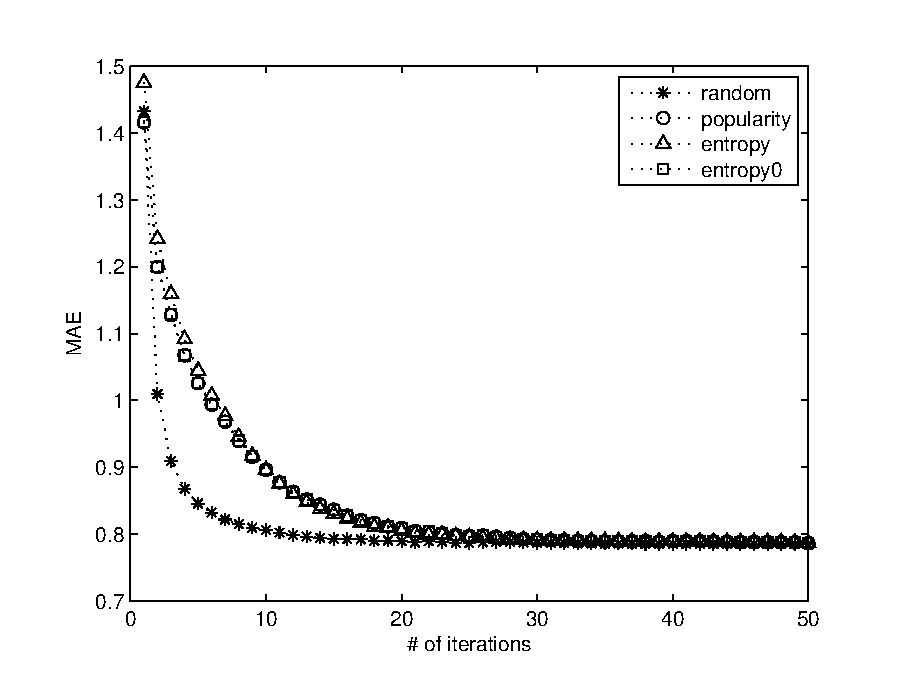
\includegraphics{ml_ent_ent0.eps}
\caption{Avaliação do grupo \textit{Entropia Pura} na base \textit{MovieLens}}
\label{fig:entropia-pura-movielens}
\end{figure}

\begin{figure}[ht]
\centering
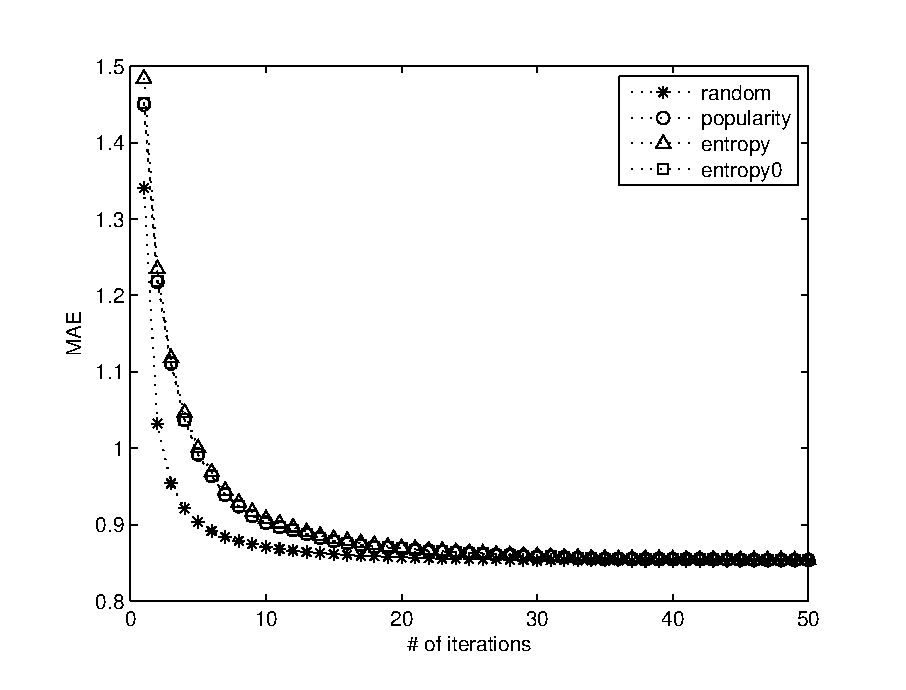
\includegraphics{nf_ent_ent0.eps}
\caption{Avaliação do grupo \textit{Entropia Pura} na base \textit{Netflix}}
\label{fig:entropia-pura-netflix}
\end{figure}

\subsection{Logaritmo da Popularidade e Entropia}

Do mesmo modo, as figuras \ref{fig:logpop-entropia-movielens} e \ref{fig:logpop-entropia-netflix} correspondem ao emprego de \textit{log(pop)*ent} e \textit{log(pop)*ent0} nas bases \textit{MovieLens} e \textit{Netflix}, respectivamente. Como é possível observar, ambas possuem comportamento muito similar a \textit{popularity}, entretanto havia indícios para suspeitarmos disso, uma vez que conhecemos os resultados do grupo \textit{Entropia Pura}.

Primeiramente, ambas estratégias estão baseadas no valor de popularidade, que representa o número de avaliações que o filme recebeu. Desta forma, tal valor, ainda que amenizado por uma função logarítmica, exerce forte influência sobre o comportamento da estratégia. Em segundo lugar, o outro componente que as compõe é o valor da entropia, dado pelas estratégias \textit{entropy} e \textit{entropy0}. É sabido que essas duas estratégias também não obtiveram comportamento muito destoante de \textit{popularity}. Logo, era esperado que tanto \textit{log(pop)*ent} como \textit{log(pop)*ent0} apresentassem comportamentos semelhantes à \textit{popularity}.

Fazendo uma analogia com o mercado de ações, podemos dizer que \textit{log(pop)*ent} está ``indexada'' por \textit{popularity} e \textit{entropy}, enquanto que \textit{log(pop)*ent0} está ``indexada'' por \textit{popularity} e \textit{entropy0}. Ou seja, assim como um fundo de investimento que está indexado por um determinado ativo (composto majoritariamente por este ativo) não apresentará rendimentos que destoam significativamente do rendimento deste ativo, da mesma maneira, o comportamento de tais estratégias não será muito distante do comportamento das suas estratégias ``índices''.

Em \citep{Elahi:2014:ALS:2542182.2542195} são apresentados apenas as estratégias \textit{log(pop)*ent} e \textit{popularity} e pode-se verificar que os comportamentos de ambas seguem bem próximos, o que confirma nossa analogia. 

\begin{figure}[ht]
\centering
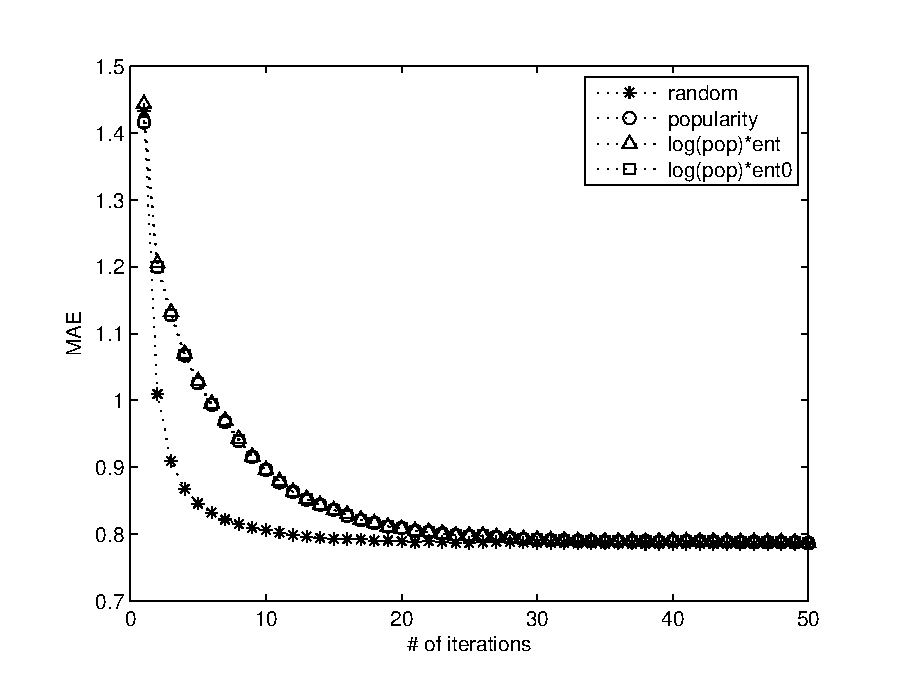
\includegraphics{ml_logpopent_logpop_ent0.eps}
\caption{Avaliação do grupo \textit{Logaritmo da Popularidade e Entropia} na base \textit{MovieLens}}
\label{fig:logpop-entropia-movielens}
\end{figure}

\begin{figure}[ht]
\centering
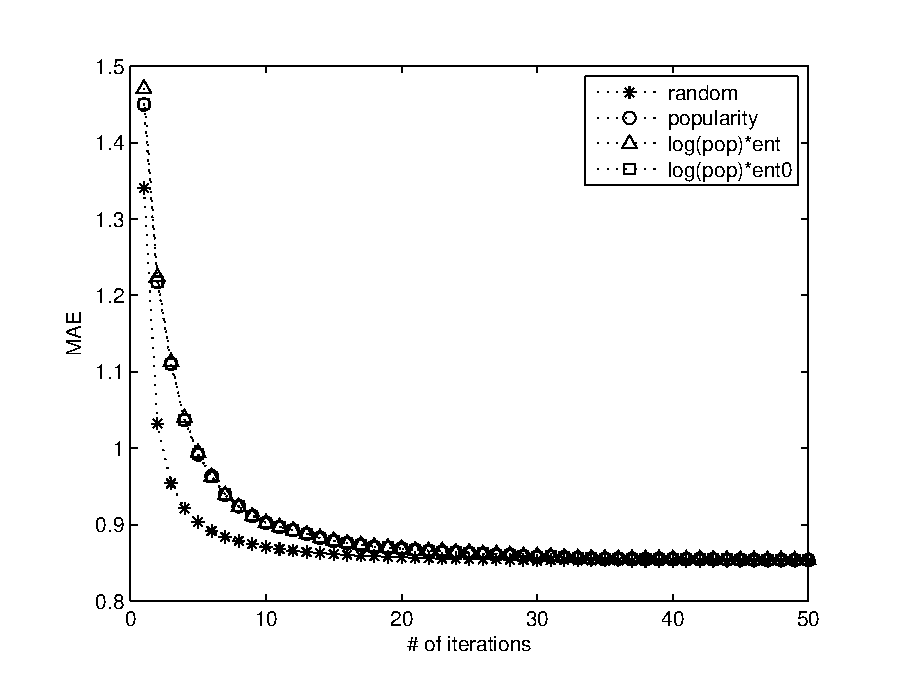
\includegraphics{nf_logpopent_logpopent0.eps}
\caption{Avaliação do grupo \textit{Logaritmo da Popularidade e Entropia} na base \textit{Netflix}}
\label{fig:logpop-entropia-netflix}
\end{figure}

\subsection{Média Harmônica da Popularidade e Entropia}

Novamente, pode-se observar a atração que as estratégias índices aplicam sobre suas indexadas. Vemos através das figuras \ref{fig:helf-movielens} e \ref{fig:helf-netflix} que \textit{helf} e \textit{helf0} recaem sobre \textit{popularity}. 

Este resultado, juntamente com o anterior, nos informa que tanto combinações simples (e.g., função logarítmica) como combinações complexas (e.g., média harmônica) não suprimem a atração que as estratégias compostas sofrem daquelas que as compõem. Concluímos então que a utilização de estratégias compostas, ou indexadas, não trará ganhos significativos quando as estratégias simples, as que lhes servem como índices, não possuem um bom comportamento elas mesmas.

Apesar de \citep{Elahi:2014:ALS:2542182.2542195} não fazer uso de \textit{helf} nem de \textit{helf0} em seus experimentos, os autores em \citep{Rashid:2008:LPN:1540276.1540302} apresentam os resultados que obtiveram com \textit{helf}. Conforme deduzido aqui, eles seguem bem próximos ao comportamento de \textit{popularity}. 

\begin{figure}[ht]
\centering
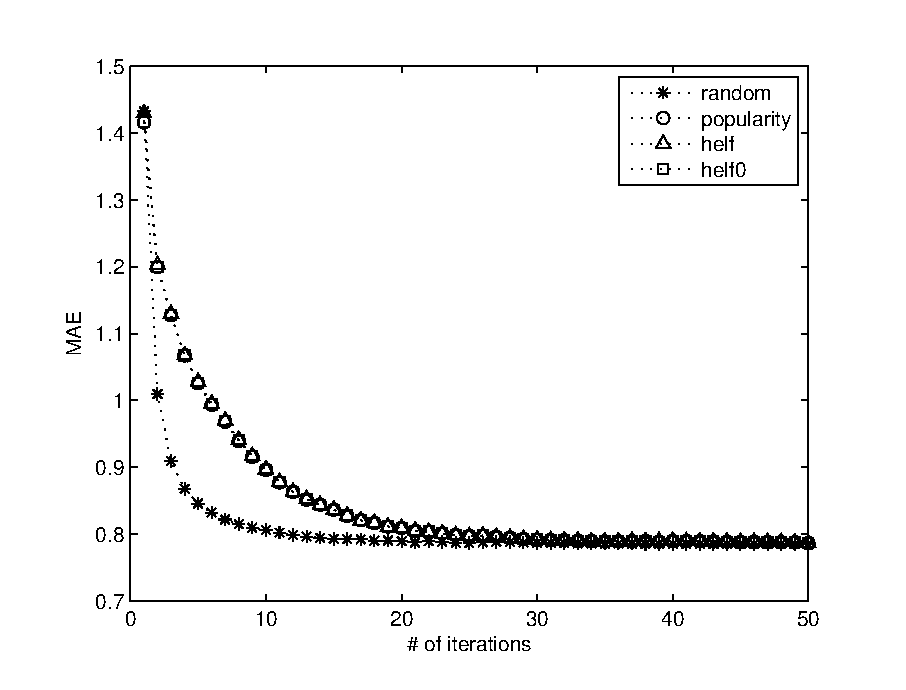
\includegraphics{ml_helf_helf0.eps}
\caption{Avaliação do grupo \textit{Média Harmônica da Popularidade e Entropia} na base \textit{MovieLens}}
\label{fig:helf-movielens}
\end{figure}

\begin{figure}[ht]
\centering
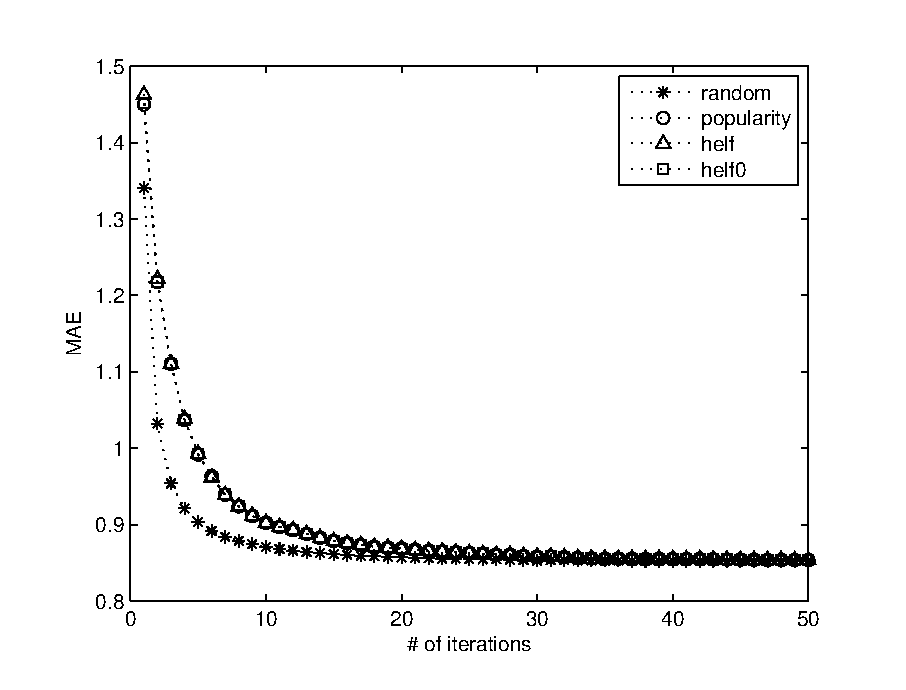
\includegraphics{nf_helf_helf0.eps}
\caption{Avaliação do grupo \textit{Média Harmônica da Popularidade e Entropia} na base \textit{Netflix}}
\label{fig:helf-netflix}
\end{figure}

\subsection{Ganho de Informação}

Dentre as estratégias da família \textit{Entropia}, \textit{igcn} parece ter obtido o melhor comportamento, conforme as figuras \ref{fig:igcn-movielens} e \ref{fig:igcn-netflix} indicam. Entretanto, mesmo sendo a melhor estratégia da família \textit{Entropia}, ela ainda fica muito aquém do desejado, que seria ultrapassar a estratégia \textit{random}.

Apesar de estar inserida nesta família, a \textit{igcn} não se baseia na entropia das preferências, mas sim na entropia dos usuários. Segundo \citep{Rashid:2008:LPN:1540276.1540302}, trabalho que propôs a estratégia, os usuários são divididos em grupos, chamados de \textit{clusters}, de acordo com suas disposições no espaço dado pela decomposição SVD. Os itens solicitados são aqueles que, se avaliados, reduzirão a incerteza associada a distribuição dos usuários em \textit{clusters}, i.e., trarão a maior redução na entropia da distribuição dos usuários.

Aqui, como no caso já comentado da entropia pura, há uma heurística subjacente à estratégia que parece introduzir viés no conjunto de treinamento. Buscar os itens com maior potencial para ``organizar'' os usuários, dentro de um espaço vetorial construído com base nas avaliações, não implica necessariamente em redução do erro do modelo. Afinal, é possível que o estado natural dos dados, incluindo as disposições dos usuários em tal espaço, seja um estado de desordem. Ao solicitar os itens que trarão uma maior organização, estamos induzindo uma ordem que é estranha aos dados e, consequentemente, podemos estar enviesando o conjunto de treinamento.

Somente \citep{Rashid:2008:LPN:1540276.1540302} apresenta resultados para \textit{igcn}, porém, infelizmente, não há comparações com \textit{random}. Todavia, faz-se comparações com \textit{helf}, \textit{entropy0} e \textit{popularity}, as quais se mostraram inferiores à \textit{igcn}, similar ao que foi verificado em nossos experimentos.

\begin{figure}[ht]
\centering
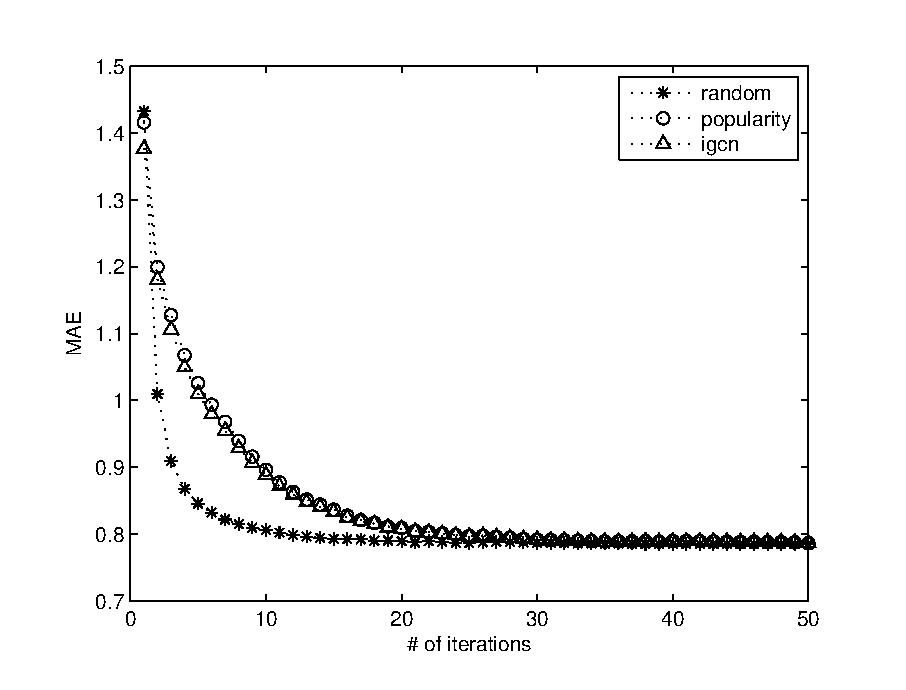
\includegraphics{ml_igcn.eps}
\caption{Avaliação do grupo \textit{Ganho de Informação} na base \textit{MovieLens}}
\label{fig:igcn-movielens}
\end{figure}

\begin{figure}[ht]
\centering
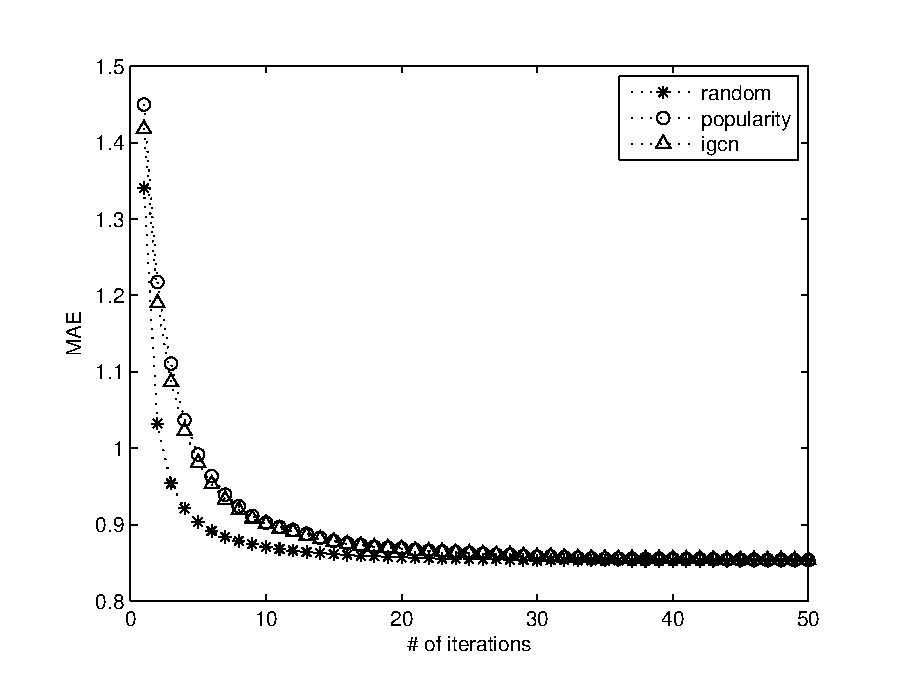
\includegraphics{nf_igcn.eps}
\caption{Avaliação do grupo \textit{Ganho de Informação} na base \textit{Netflix}}
\label{fig:igcn-netflix}
\end{figure}

\section{Variância}

Na família \textit{Variância}, como há apenas três estratégias, decidimos por não dividir em grupos e apresentá-las todas de uma só vez. Os resultados podem ser vistos nas figuras \ref{fig:variance-movielens} e \ref{fig:variance-netflix}, paras as bases \textit{Movielens} e \textit{Netflix}, respectivamente.

Vemos que a estratégias \textit{variance} apresenta uma ligeira vantagem sobre as demais, sobretudo na figura \ref{fig:variance-movielens}, nas primeiras 10 iterações. Contudo, seu comportamento passa logo a seguir o de \textit{popularity}, o que aponta para a presença de viés em $K$. Novamente, como no caso da entropia, tentar minimizar a incerteza dos itens através da variância, acarreta na construção de um conjunto de treinamento dominado pelos itens mais controversos. Tais itens são justamente os mais difíceis de se prever avaliações e, portanto, o modelo tem grande dificuldade em capturar o padrão que determina as avaliações dadas pelos usuários.  

As estratégias compostas utilizando \textit{variance} e \textit{popularity} caem no mesmo inconveniente das estratégias compostas que fazem uso de \textit{entropy} (ou \textit{entropy0}) e \textit{popularity}, ou seja, acabam por serem atraídas para o comportamento de \textit{popularity}. O que explica a semelhança de comportamento tanto de \textit{log(pop)*var} de \textit{sqrt(pop)*var} com \textit{popularity}.

\begin{figure}[ht]
\centering
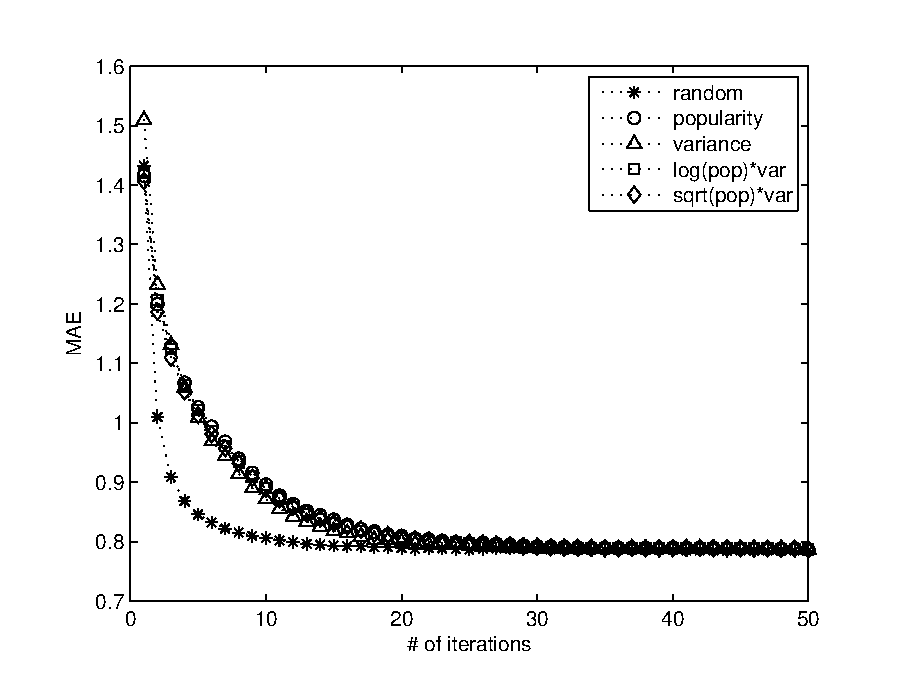
\includegraphics{ml_variance_family.eps}
\caption{Avaliação da família \textit{Variância} na base \textit{MovieLens}}
\label{fig:variance-movielens}
\end{figure}

\begin{figure}[ht]
\centering
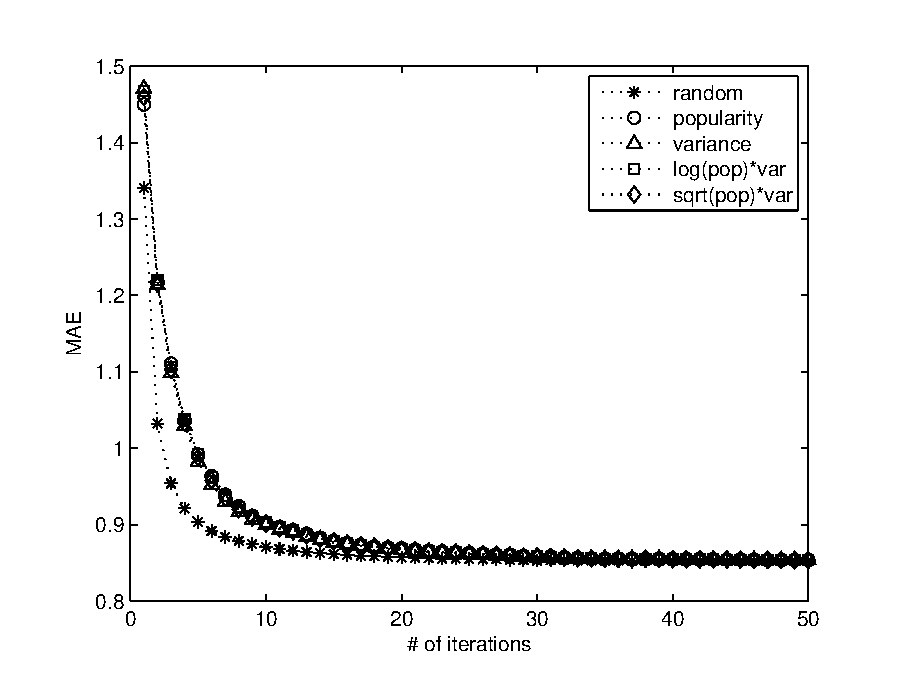
\includegraphics{nf_variance_family.eps}
\caption{Avaliação da família \textit{Variância} na base \textit{Netflix}}
\label{fig:variance-netflix}
\end{figure}

\section{Modelo}

Dentre as estratégias da família \textit{Modelo}, duas delas obtiveram desempenho pior que a estratégia \textit{random}, enquanto que as outras duas foram melhores. Aliás, deve-se mencionar que foram as únicas de todo nosso experimento que conseguiram tal feitio, com exceção da \textit{Estratégia Livre de Viés}. Cabe à nós então analisarmos o porquê deste comportamento inusitado, tendo sempre em mente a heurística por trás de cada estratégia.

\subsection{Pior que \textit{random}}

Começaremos por analisar as estratégias que obtiveram desempenho pior que \textit{random}, isto é, \textit{high pred} e \textit{bin pred}, exibidas nas figuras \ref{fig:worst-random-movielens} e \ref{fig:worst-random-netflix}. Observamos que ambas, até a 10ª iteração, apresentam desempenho ligeiramente superior à \textit{popularity}, convergindo mais tarde para o comportamento desta.

É importante levar em consideração que ambas as bases contêm preferências em forma de números inteiros, variando de 1 a 5. Das 100 mil avaliações presentes na base \textit{MovieLens}, cerca de 6\% das notas possuem valor igual a 1; 12\% igual a 2; 27\% igual a 3; 34\% igual a 4; e 21\% igual 5. Na base \textit{Netflix}, por sua vez, das 100 mil avaliações, cerca de 8\% possuem valor igual a 1; 14\% igual a 2; 35\% igual a 3; 27\% igual a 4; e 16\% igual a 5.

Se considerarmos as notas 1 e 2 como avaliações ``baixas'', e as notas 3, 4 e 5 como avaliações ``altas'', verificamos que \textit{MovieLens} e \textit{Netflix} possuem 82\% e 78\% das notas como sendo altas, respectivamente. Esta característica pode elucidar muito a respeito do desempenho que tais estratégias tiveram nessas bases.

A estratégia \textit{high pred} busca solicitar os itens que receberam as melhores previsões do modelo, ou seja, itens cujas previsões apontam para preferências altas. Desta maneira, ela insere no conjunto de treinamento $K$ sempre preferências altas, agravando o desequilíbrio natural que existe entre as preferências e tornando o conjunto ainda mais desbalanceado. Como o modelo é treinado com as preferências em $K$, este desequilíbrio transfere-se para a acurácia do mesmo, que acaba por ficar mais preciso em prever preferências altas do que baixas.

Por sua vez, \textit{bin pred} procura inserir em $K$ os itens cujas previsões apontam para alguma preferência, seja ela baixa ou alta. Em outras palavras, \textit{bin pred} solicita os itens cujas previsões indicam que os mesmos serão ``consumidos''. Esta abordagem não faz distinção entre as preferências, reduzindo-as a simples informações binárias. Com isso, acabamos simplesmente mantendo o desequilíbrio natural das preferências, visto que, ao contrário do caso de \textit{high pred}, não temos nenhuma ideia de como o usuário avaliará os itens solicitados.

Ambas as estratégias apresentam desempenho ruim em \citep{Elahi:2014:ALS:2542182.2542195}, ou seja, pior que \textit{random}. Contudo, no referido trabalho, \textit{bin pred} é nitidamente melhor que \textit{high pred}, o que não ficou claro em nossos experimentos. Na medida em que solicita apenas os itens de previsão alta, \textit{high pred} reforça o desequilíbrio entre as preferências em $K$, agravando a disparidade entre as previsões. Como \textit{bin pred} não sabe qual foi o valor efetivo da preferência prevista, o desequilíbrio em $K$ apenas se mantem com os itens solicitados. Por exemplo, mesmo que haja itens com previsão alta, é possível que \textit{bin pred} solicite itens com previsão baixa, o que não seria possível em \textit{high pred}.  

\begin{figure}[ht]
\centering
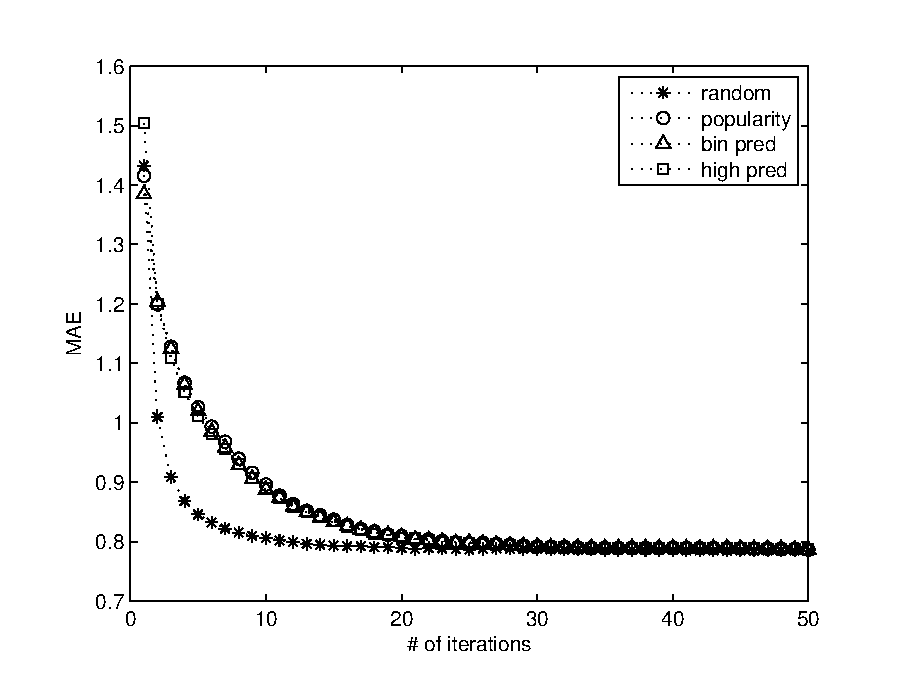
\includegraphics{ml_bin_high.eps}
\caption{Avaliação do grupo \textit{Pior que random} na base \textit{MovieLens}}
\label{fig:worst-random-movielens}
\end{figure}

\begin{figure}[ht]
\centering
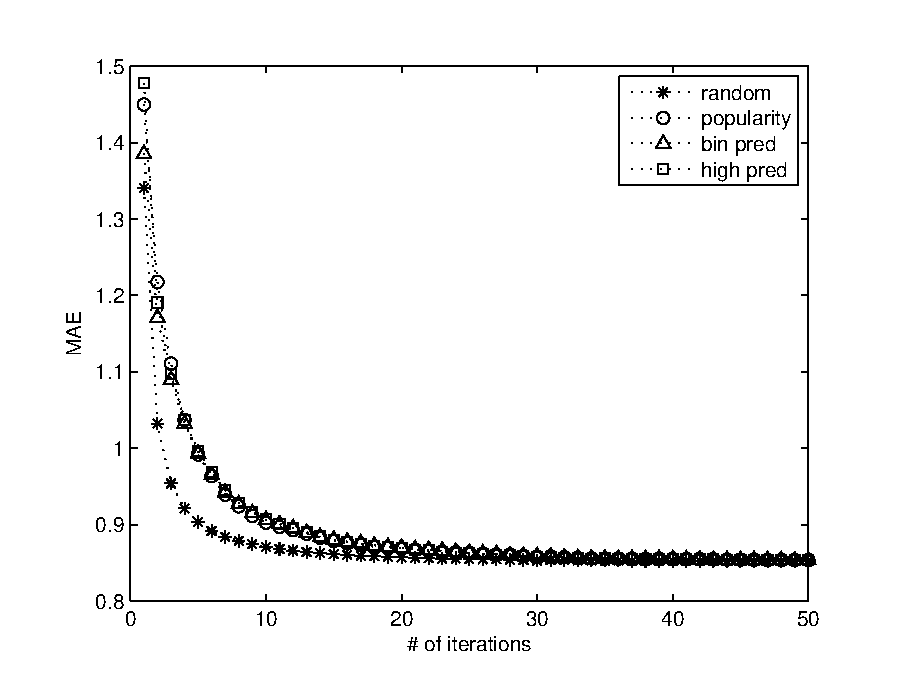
\includegraphics{nf_bin_high.eps}
\caption{Avaliação do grupo \textit{Pior que random} na base \textit{Netflix}}
\label{fig:worst-random-netflix}
\end{figure}

\subsection{Melhor que \textit{random}}
\label{sec:melhor-random}

As únicas estratégias que obtiveram desempenho melhor que \textit{random}, com exceção da \textit{Estratégia Livre de Viés}, foram \textit{low pred} e \textit{high-low pred}, conforme pode ser observado nas figuras \ref{fig:better-random-movielens} e \ref{fig:better-random-netflix}.

Ao contrário de \textit{high pred}, \textit{low pred} busca solicitar os itens cujas previsões apontam para preferências baixas. Uma vez que há uma carência natural por tais preferências, ao solicitá-las, esta estratégia introduz em $K$ justamente as preferências faltantes, amenizando o desequilíbrio entre preferências baixas e altas. O conjunto de treinamento acaba ficando mais equilibrado e, consequentemente, a acurácia do modelo fica mais balanceada, capaz de fazer previsões mais precisas para todos os tipos de preferência. 

Ou seja, a estratégia \textit{low pred} se beneficia da carência natural de preferências baixas. A heurística que a norteia, solicitar os itens com previsões baixas, mostrou-se eficaz visto que as bases utilizadas em nossos experimentos carecem de tais preferências. Caso as características das bases fossem outras ou se modificassem com o tempo, o desempenho da estratégia poderia ser diferente. Em outras palavras, o simples fato de que a estratégia obteve um bom desempenho não significa que ela não introduz viés no conjunto de treinamento. Pelo contrário, a própria concepção da estratégia implica na construção de um conjunto de treinamento enviesado, porém, neste caso, o viés nos foi útil.

Da mesma forma, \textit{high-low pred} assume que é preferível solicitar itens cujas previsões se distanciam do valor médio de preferência. Em ambas as bases, as avaliações podem possuir valores inteiros de 1 a 5, sendo o valor médio 3. Logo, \textit{high-low pred} procura solicitar itens cuja previsão é igual a 1 ou 5 (valores mais distantes do valor médio). Se definirmos as notas 1 e 5 como sendo avaliações ``extremas'' e as notas 2, 3, e 4 como avaliações ``medianas'', constatamos que 73\% das avaliações em \textit{MovieLens} são medianas, enquanto que, em \textit{Netflix}, este percentual é de 76\%.

Ou seja, a distinção entre avaliações baixas e altas esconde um pouco o verdadeiro desequilíbrio entre as preferências. Na verdade, as notas 3 e 4 compõem a grande maioria das avaliações nas duas bases, sendo 61\% das avaliações em \textit{MovieLens} e 62\% em \textit{Netflix}. Assim como \textit{low pred}, ao solicitar os itens cujas previsões apontam para preferências extremas, \textit{high-low pred} ameniza o desequilíbrio natural que existe nas bases e promove um treinamento mais balanceado do modelo. A heurística subjacente à estratégia acaba sendo, mais uma vez, útil, pois ataca justamente a desproporção entre as preferências. 

Em \citep{Elahi:2014:ALS:2542182.2542195}, tanto \textit{low pred} quanto \textit{high-low pred} apresentam desempenho pior que \textit{random} nas primeiras iterações, porém conseguem alcançar e superar esta estratégia. No entanto, \textit{high-low pred} mostrou-se melhor que \textit{low pred}, o que não ficou claro em nosso trabalho. Isto significa que a distinção entre preferências ``extremas'' e ``medianas'' representa melhor a realidade dos dados do que a distinção entre preferências ``baixas'' e ``altas''. 

%O bom desempenho de \textit{high-low pred}, por sua vez, pode ser explicado pelo mesmo argumento utilizado para justificar o desempenho das estratégias indexadas (e.g., \textit{helf}, \textit{log(pop)*ent0}, etc.). Isto é, como \textit{high-low pred} está indexada por \textit{low pred}, o comportamento da estratégia índice acaba por atrair o comportamento da indexada.
%O curioso de notar neste caso é que \textit{high-low pred} também está indexa por \textit{high pred}, que, por sua vez, não obteve um bom desempenho. Assim, temos motivos para supor que uma estratégia indexada por duas ou mais estratégias será atraída mais fortemente pela estratégia índice com melhor desempenho, contudo, maiores evidências se fazem necessárias para que possamos concluir de fato esta propriedade. Verificamos que \textit{low pred} e \textit{high-low pred} apresentam comportamentos semelhantes em \citep{Elahi:2014:ALS:2542182.2542195}, o que traz mais crédito à nossa análise.

\begin{figure}[ht]
\centering
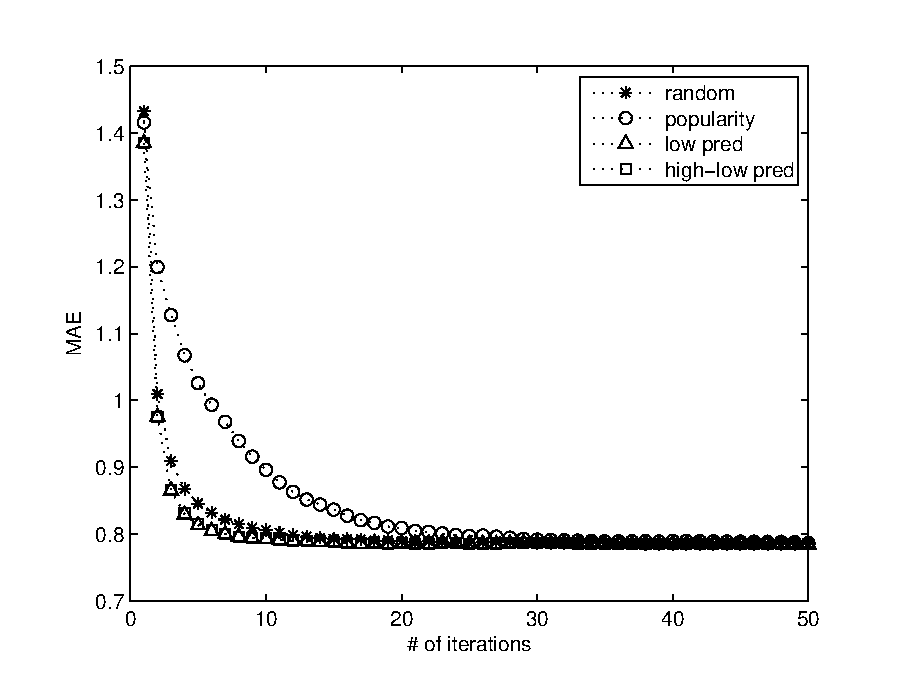
\includegraphics{ml_low_highlow.eps}
\caption{Avaliação do grupo \textit{Melhor que random} na base \textit{MovieLens}}
\label{fig:better-random-movielens}
\end{figure}

\begin{figure}[ht]
\centering
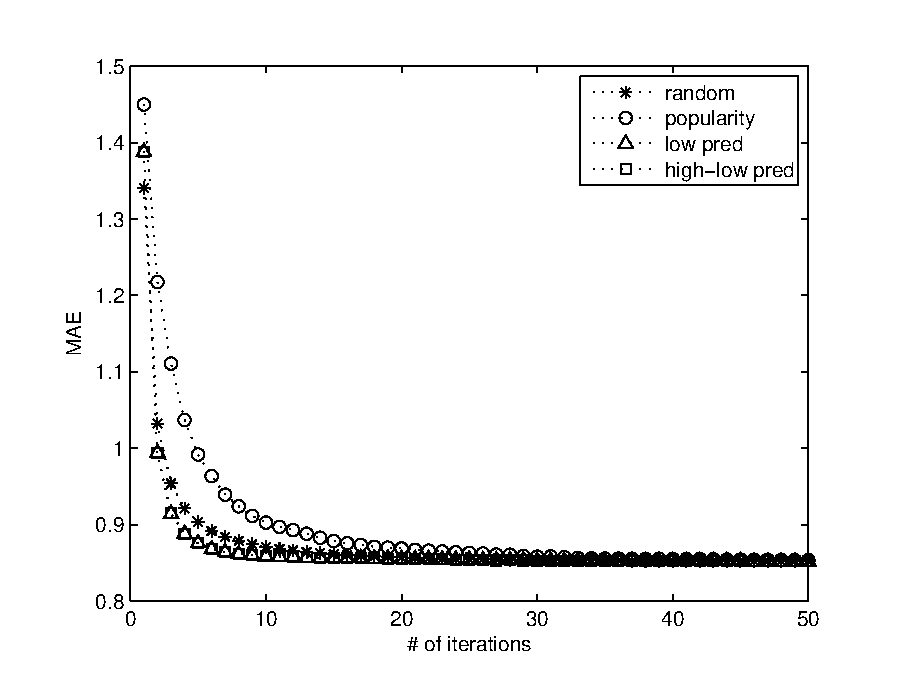
\includegraphics{nf_low_highlow.eps}
\caption{Avaliação do grupo \textit{Melhor que random} na base \textit{Netflix}}
\label{fig:better-random-netflix}
\end{figure}

\section{Estratégia Livre de Viés}

Iremos analisar nas próximas seções o comportamento da \textit{Estratégia Livre de Viés}, nomeada como \textit{unbiased} em nossos experimentos, comparando seu comportamento com as duas melhores estratégias até então: \textit{low pred} e \textit{high-low pred}. Além de uma análise global, visualizando todas as iterações, optamos também por realizar uma análise ampliada, com foco nas primeiras 15 primeiras iterações, onde é possível perceber mais nitidamente a superioridade de \textit{unbiased}.

\subsection{\textit{unbiased vs. low pred}}

As figuras \ref{fig:unbiased-lowpred-global-movielens} e \ref{fig:unbiased-lowpred-global-netflix} apresentam uma visão global, ou seja, uma visualização dos comportamentos de \textit{low pred} e \textit{unbiased} durante todas as iterações, nas bases \textit{MovieLens} e \textit{Netflix}, respectivamente. É possível verificar que, nas duas primeiras iterações, \textit{low pred} apresenta certa vantagem, entretanto, a partir da 3ª iteração, \textit{unbiased} parece alcançá-la e acompanhá-la até o final. Infelizmente, como o ganho de \textit{unbiased} é muito sutil, não conseguimos percebê-lo nesta escala.

Assim, decidimos por apresentar uma visão ampliada dos comportamentos de \textit{low pred} e \textit{unbiased}, até a 15ª iteração, de modo que seja possível visualizar com clareza a vantagem desta última. As figuras \ref{fig:unbiased-lowpred-focus-movielens} e \ref{fig:unbiased-lowpred-focus-netflix} exibem esta visão ampliada nas bases \textit{MovieLens} e \textit{Netflix}, respectivamente.

Vemos que \textit{unbiased} começa pior que \textit{low pred} em ambas as bases, porém, passadas algumas iterações, a primeira alcança a segunda e a supera. É interessante notar que, na base \textit{MovieLens}, \textit{unbiased} alcança \textit{low pred} já na 3ª iteração, enquanto que, em \textit{Netflix}, o empate só se dá por volta da 9ª iteração. Contudo, após o ponto de empate, em ambas as bases, pode-se observar que \textit{unbiased} toma a preeminência sobre a acurácia.

Um detalhe interessante é que esta preeminência de \textit{unbiased} é muito mais explícita na base \textit{MovieLens} do que na base \textit{Netflix}. Além do ponto de empate ocorrer mais cedo, o desvio padrão da acurácia, denotado pelas barras verticais, de \textit{unbiased} está abaixo do de \textit{low pred} em \textit{MovieLens} e eles não se sobrepõem. Isto significa que, mesmo no seu pior momento, o desempenho de \textit{unbiased} ainda é melhor do que o melhor momento de \textit{low pred}.

Embora este resultado nos remeta a conclusão de que \textit{unbiased} é efetivamente melhor que \textit{low pred}, é preciso lembrar que nossas conclusões devem se limitar ao dados em questão. Ou seja, apesar do comportamento de \textit{unbiased} ser nitidamente melhor que \textit{low pred}, na base \textit{MovieLens}, os resultados na base \textit{Netflix} já nos levam a uma conclusão diferente. Na média, o comportamento de \textit{unbiased} até foi superior ao de \textit{low pred} em \textit{Netflix}, no entanto, vemos que o desvio padrão das duas estratégias sobrepõem-se nesta base, o que indica que \textit{low pred}, em seus melhores momentos, pode superar \textit{unbiased}. 

Esta superioridade de \textit{unbiased} em \textit{MovieLens} pode ser explicada pelo fato de que a escolha dos parâmetros de \textit{unbiased} foi realizada com base apenas em \textit{MovieLens}. É possível que, utilizando parâmetros diferentes, possamos atingir resultados em \textit{Netflix} similares aos de \textit{MovieLens}. 

\begin{figure}[ht]
\centering
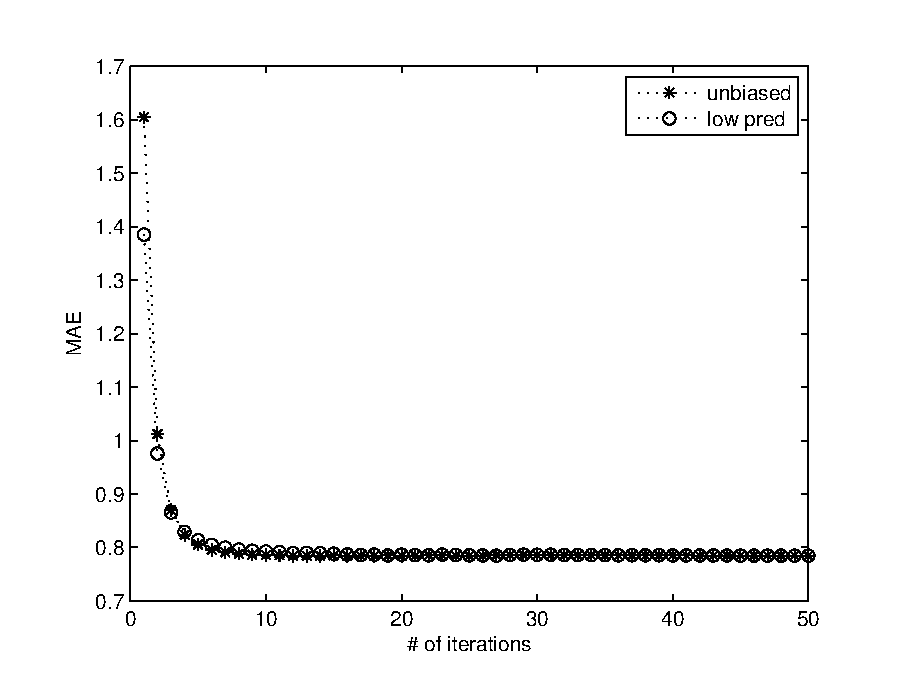
\includegraphics{ml_global_low_unbiased.eps}
\caption{Visão global de \textit{unbiased vs. low pred}  na base \textit{MovieLens}}
\label{fig:unbiased-lowpred-global-movielens}
\end{figure}

\begin{figure}[ht]
\centering
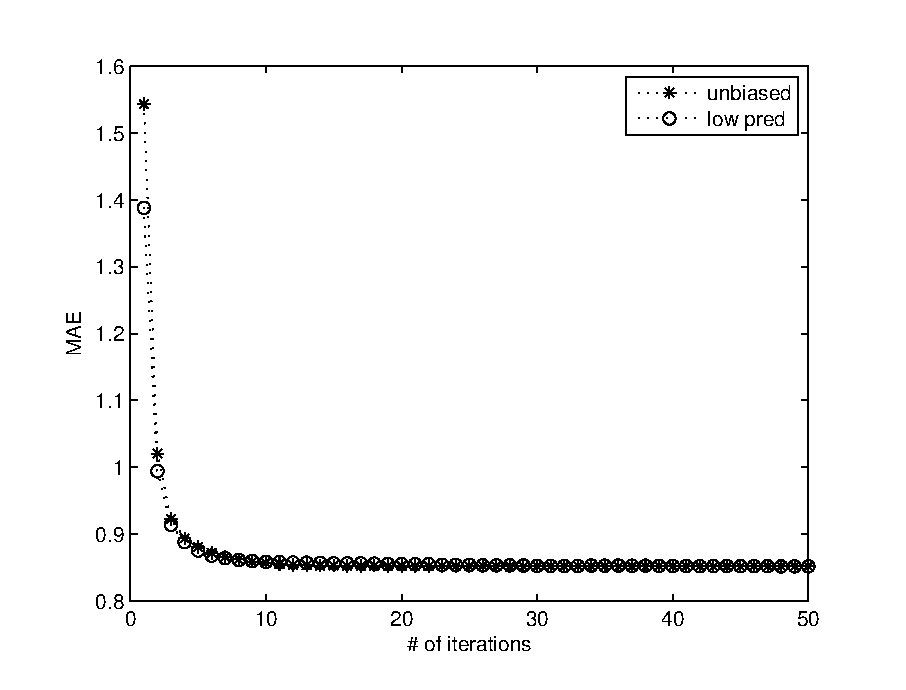
\includegraphics{nf_global_low_unbiased.eps}
\caption{Visão global de \textit{unbiased vs. low pred} na base \textit{Netflix}}
\label{fig:unbiased-lowpred-global-netflix}
\end{figure}

\begin{figure}[ht]
\centering
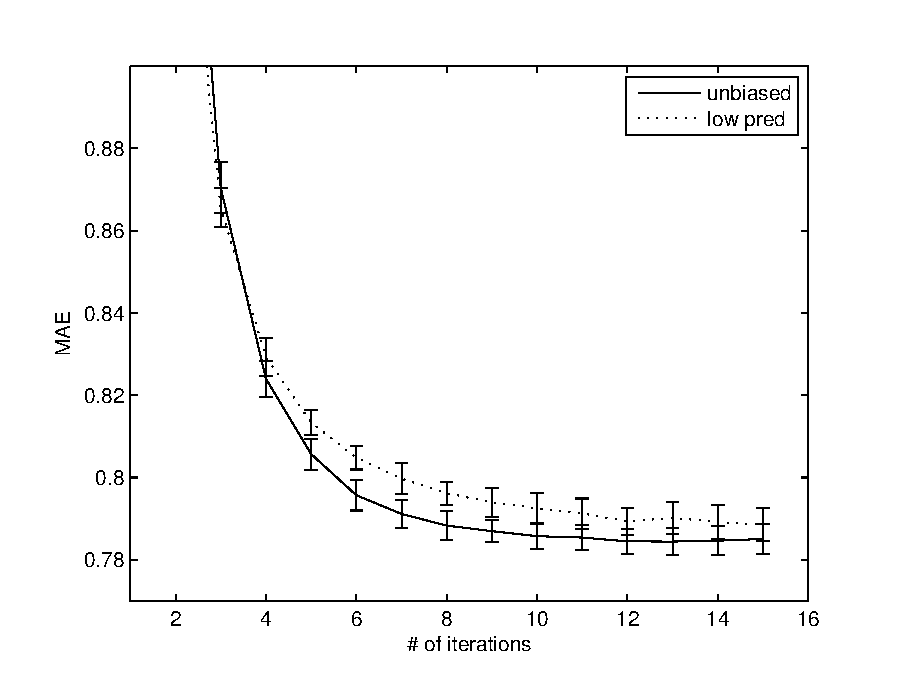
\includegraphics{ml_focus_low_unbiased.eps}
\caption{Visão ampliada de \textit{unbiased vs. low pred} na base \textit{MovieLens}}
\label{fig:unbiased-lowpred-focus-movielens}
\end{figure}

\begin{figure}[ht]
\centering
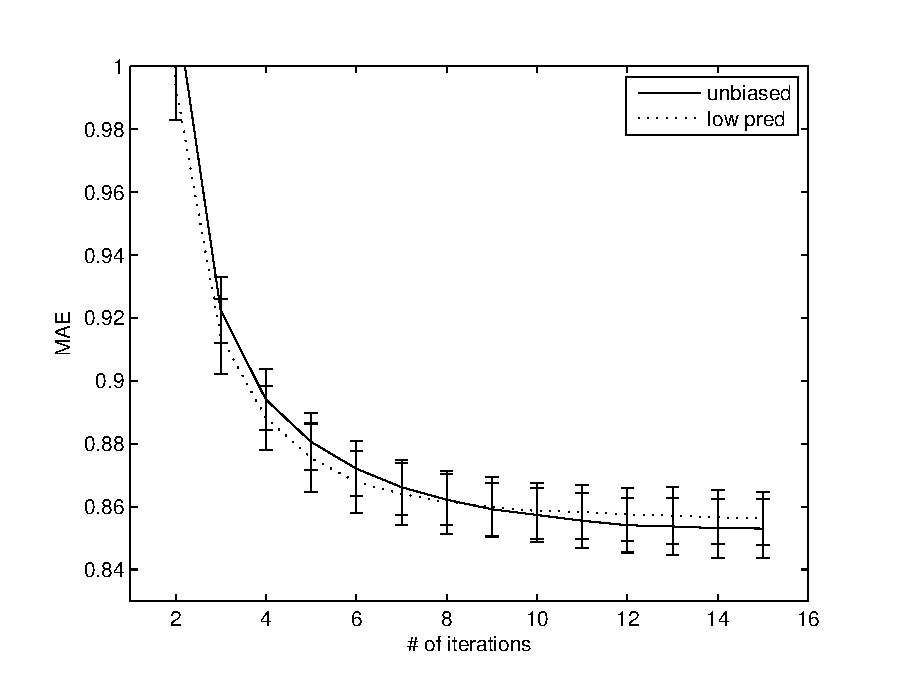
\includegraphics{nf_focus_low_unbiased.eps}
\caption{Visão ampliada de \textit{unbiased vs. low pred} na base \textit{Netflix}}
\label{fig:unbiased-lowpred-focus-netflix}
\end{figure}

\subsection{\textit{unbiased vs. high-low pred}}

Quando comparamos \textit{unbiased} com \textit{high-low pred} encontramos resultados muito parecidos com a comparação feita com \textit{low pred}. As figuras \ref{fig:unbiased-highlowpred-global-movielens} e \ref{fig:unbiased-highlowpred-global-netflix} exibem a visão global para as bases \textit{MovieLens} e \textit{Netflix}, respectivamente. Através delas, observa-se que, em ambas as bases, \textit{unbiased} começa com uma notória desvantagem frente a \textit{high-low pred}, porém, já na 3ª iteração, ambas parecem confluir para um mesmo valor e seguem assim até o final do experimento.

Na visão ampliada para as bases \textit{MovieLens} e \textit{Netflix}, obtida através das figuras \ref{fig:unbiased-highlowpred-focus-movielens} e \ref{fig:unbiased-highlowpred-focus-netflix}, respectivamente, vê-se que o ponto de empate de \textit{unbiased} e \textit{high-low pred}, em \textit{MovieLens}, se dá pela 3ª iteração, enquanto que, em \textit{Netflix}, este ponto se dá pela 9ª iteração. Além disso, a relação entre os desvios padrão também se mantem a mesma, já que em \textit{MovieLens} não há sobreposição e em \textit{Netflix} há.

De fato, não deveríamos esperar um resultado diferente para a comparação com \textit{high-low pred}. Tanto \textit{low pred} e \textit{high-low pred} se baseiam em heurísticas que procuram tornar o conjunto de treinamento mais balanceado. \textit{low pred} dá prioridade a itens com previsões 1 e 2 por serem avaliações ``baixas'', enquanto que \textit{high-low pred} também dá prioridade a itens com previsão 1 e 2 por serem ``extremas''. Assim, é esperado que haja uma enorme interseção dos itens solicitados por ambas as estratégias e, consequentemente, uma sintonia muito forte de seus comportamentos. Além disso, a questão dos parâmetros também influencia a obtenção do melhor resultado em \textit{MovieLens}.

\begin{figure}[ht]
\centering
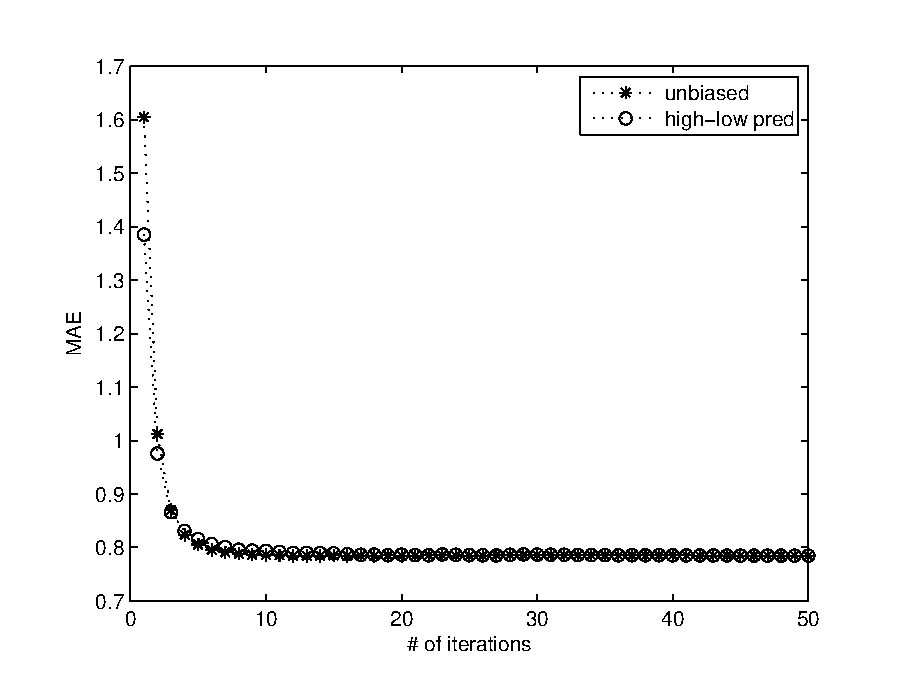
\includegraphics{ml_global_highlow_unbiased.eps}
\caption{Visão global de \textit{unbiased vs. high-low pred}  na base \textit{MovieLens}}
\label{fig:unbiased-highlowpred-global-movielens}
\end{figure}

\begin{figure}[ht]
\centering
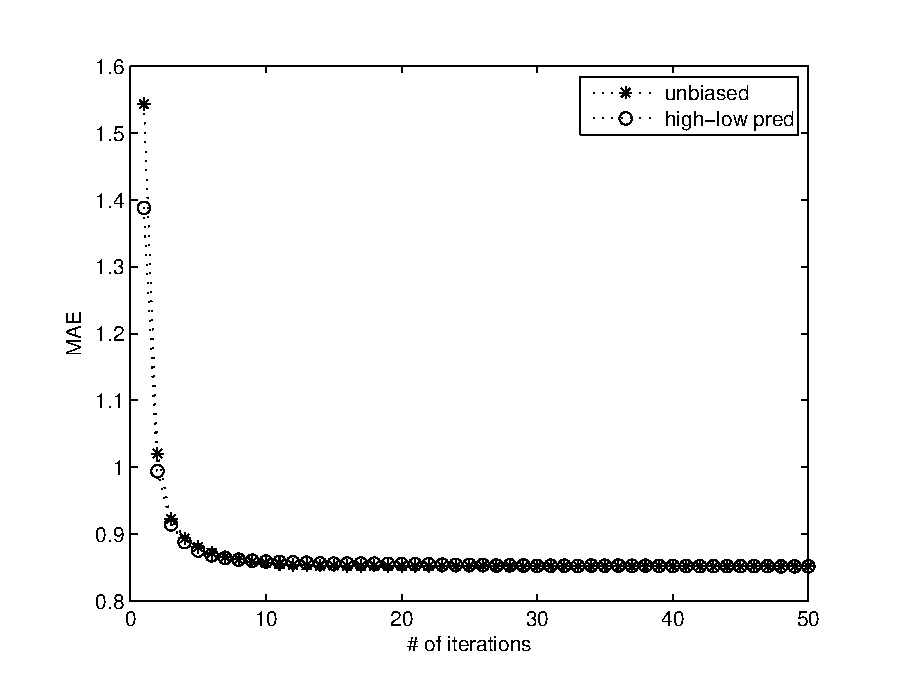
\includegraphics{nf_global_highlow_unbiased.eps}
\caption{Visão global de \textit{unbiased vs. high-low pred} na base \textit{Netflix}}
\label{fig:unbiased-highlowpred-global-netflix}
\end{figure}

\begin{figure}[ht]
\centering
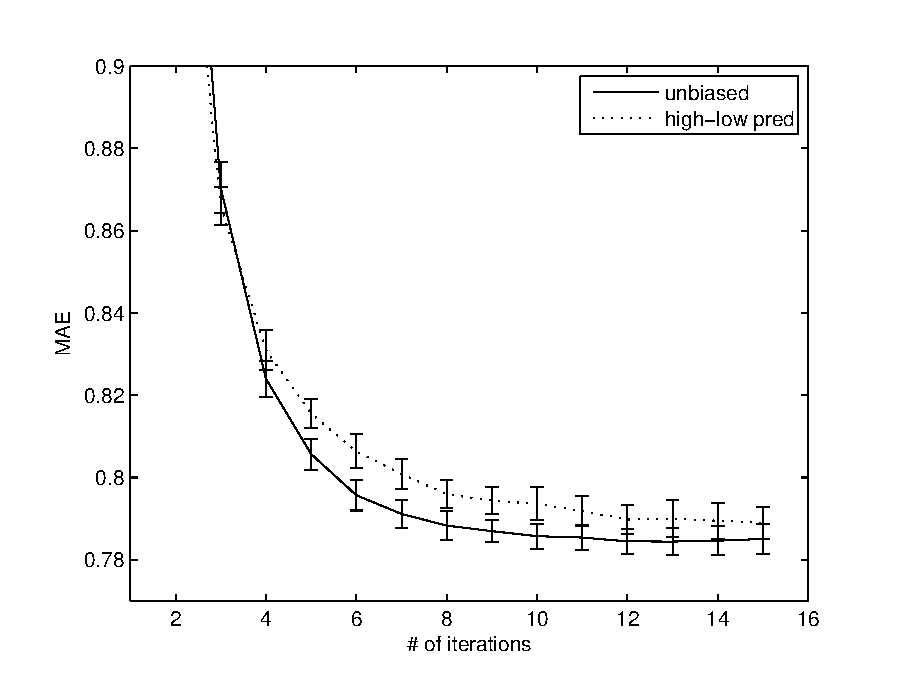
\includegraphics{ml_focus_highlow_unbiased.eps}
\caption{Visão ampliada de \textit{unbiased vs. high-low pred} na base \textit{MovieLens}}
\label{fig:unbiased-highlowpred-focus-movielens}
\end{figure}

\begin{figure}[ht]
\centering
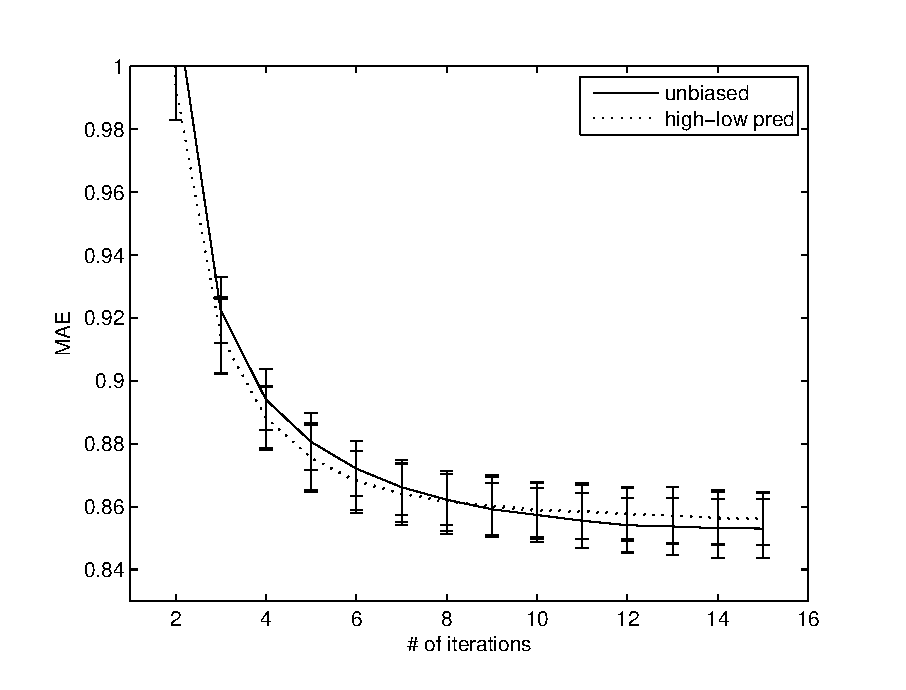
\includegraphics{nf_focus_highlow_unbiased.eps}
\caption{Visão ampliada de \textit{unbiased vs. high-low pred} na base \textit{Netflix}}
\label{fig:unbiased-highlowpred-focus-netflix}
\end{figure}